\documentclass[a4j,10pt,twocolumn]{extarticle}

% ---------------

\usepackage{report_template}
\usepackage{amsmath}
\usepackage{amssymb}
\usepackage{ascmac}
\usepackage{latexsym}
\usepackage{ulem}
\usepackage[dvipdfmx]{graphicx}
\usepackage{enumitem}
\usepackage{pifont}
\usepackage{pifont}
\usepackage[ja]{datetime2}
\usepackage{hyperref}
\newcommand{\textfilledsquare}{\ding{110}}

%%　インデントの設定
\setlist[itemize,1]{label=\scalebox{2.0}\textbullet, leftmargin=2.3em, labelsep=0.5em, align=parleft}
\setlist[itemize,2]{label=\scalebox{0.7}{○}, leftmargin=2.0em, labelsep=0.5em, align=parleft}
\setlist[itemize,3]{label=\scalebox{0.5}\textfilledsquare, leftmargin=3.0em, labelsep=0.5em, align=parleft}

% ---------------

%% 題目
\title{進捗報告テンプレート}

%% 著者
\author{神田　翼}

\begin{document}
\maketitle
\thispagestyle{empty}	% 1ページ目のページ番号を表示しない
% ------------------------------------------------------------
\the\year 年 \the\month 月 \the\day 日 \par
\vskip 1.0em
以下のようなスタイルで作ってみました．自身が使いやすいように適宜変更してください．
\section{進捗報告}
\begin{itemize}
  \item 東大阪
  \begin{itemize}
    \item 人感センサの検証
    \begin{itemize}
      \item 人感センサの検知範囲縮小のために作ったカバーの検証中\cite{1}．(図\ref{Fig:PIRsensor},表\ref{Tab:range})
    \end{itemize}
  \end{itemize}
\end{itemize}


\begin{figure}[h]
  \begin{center}
  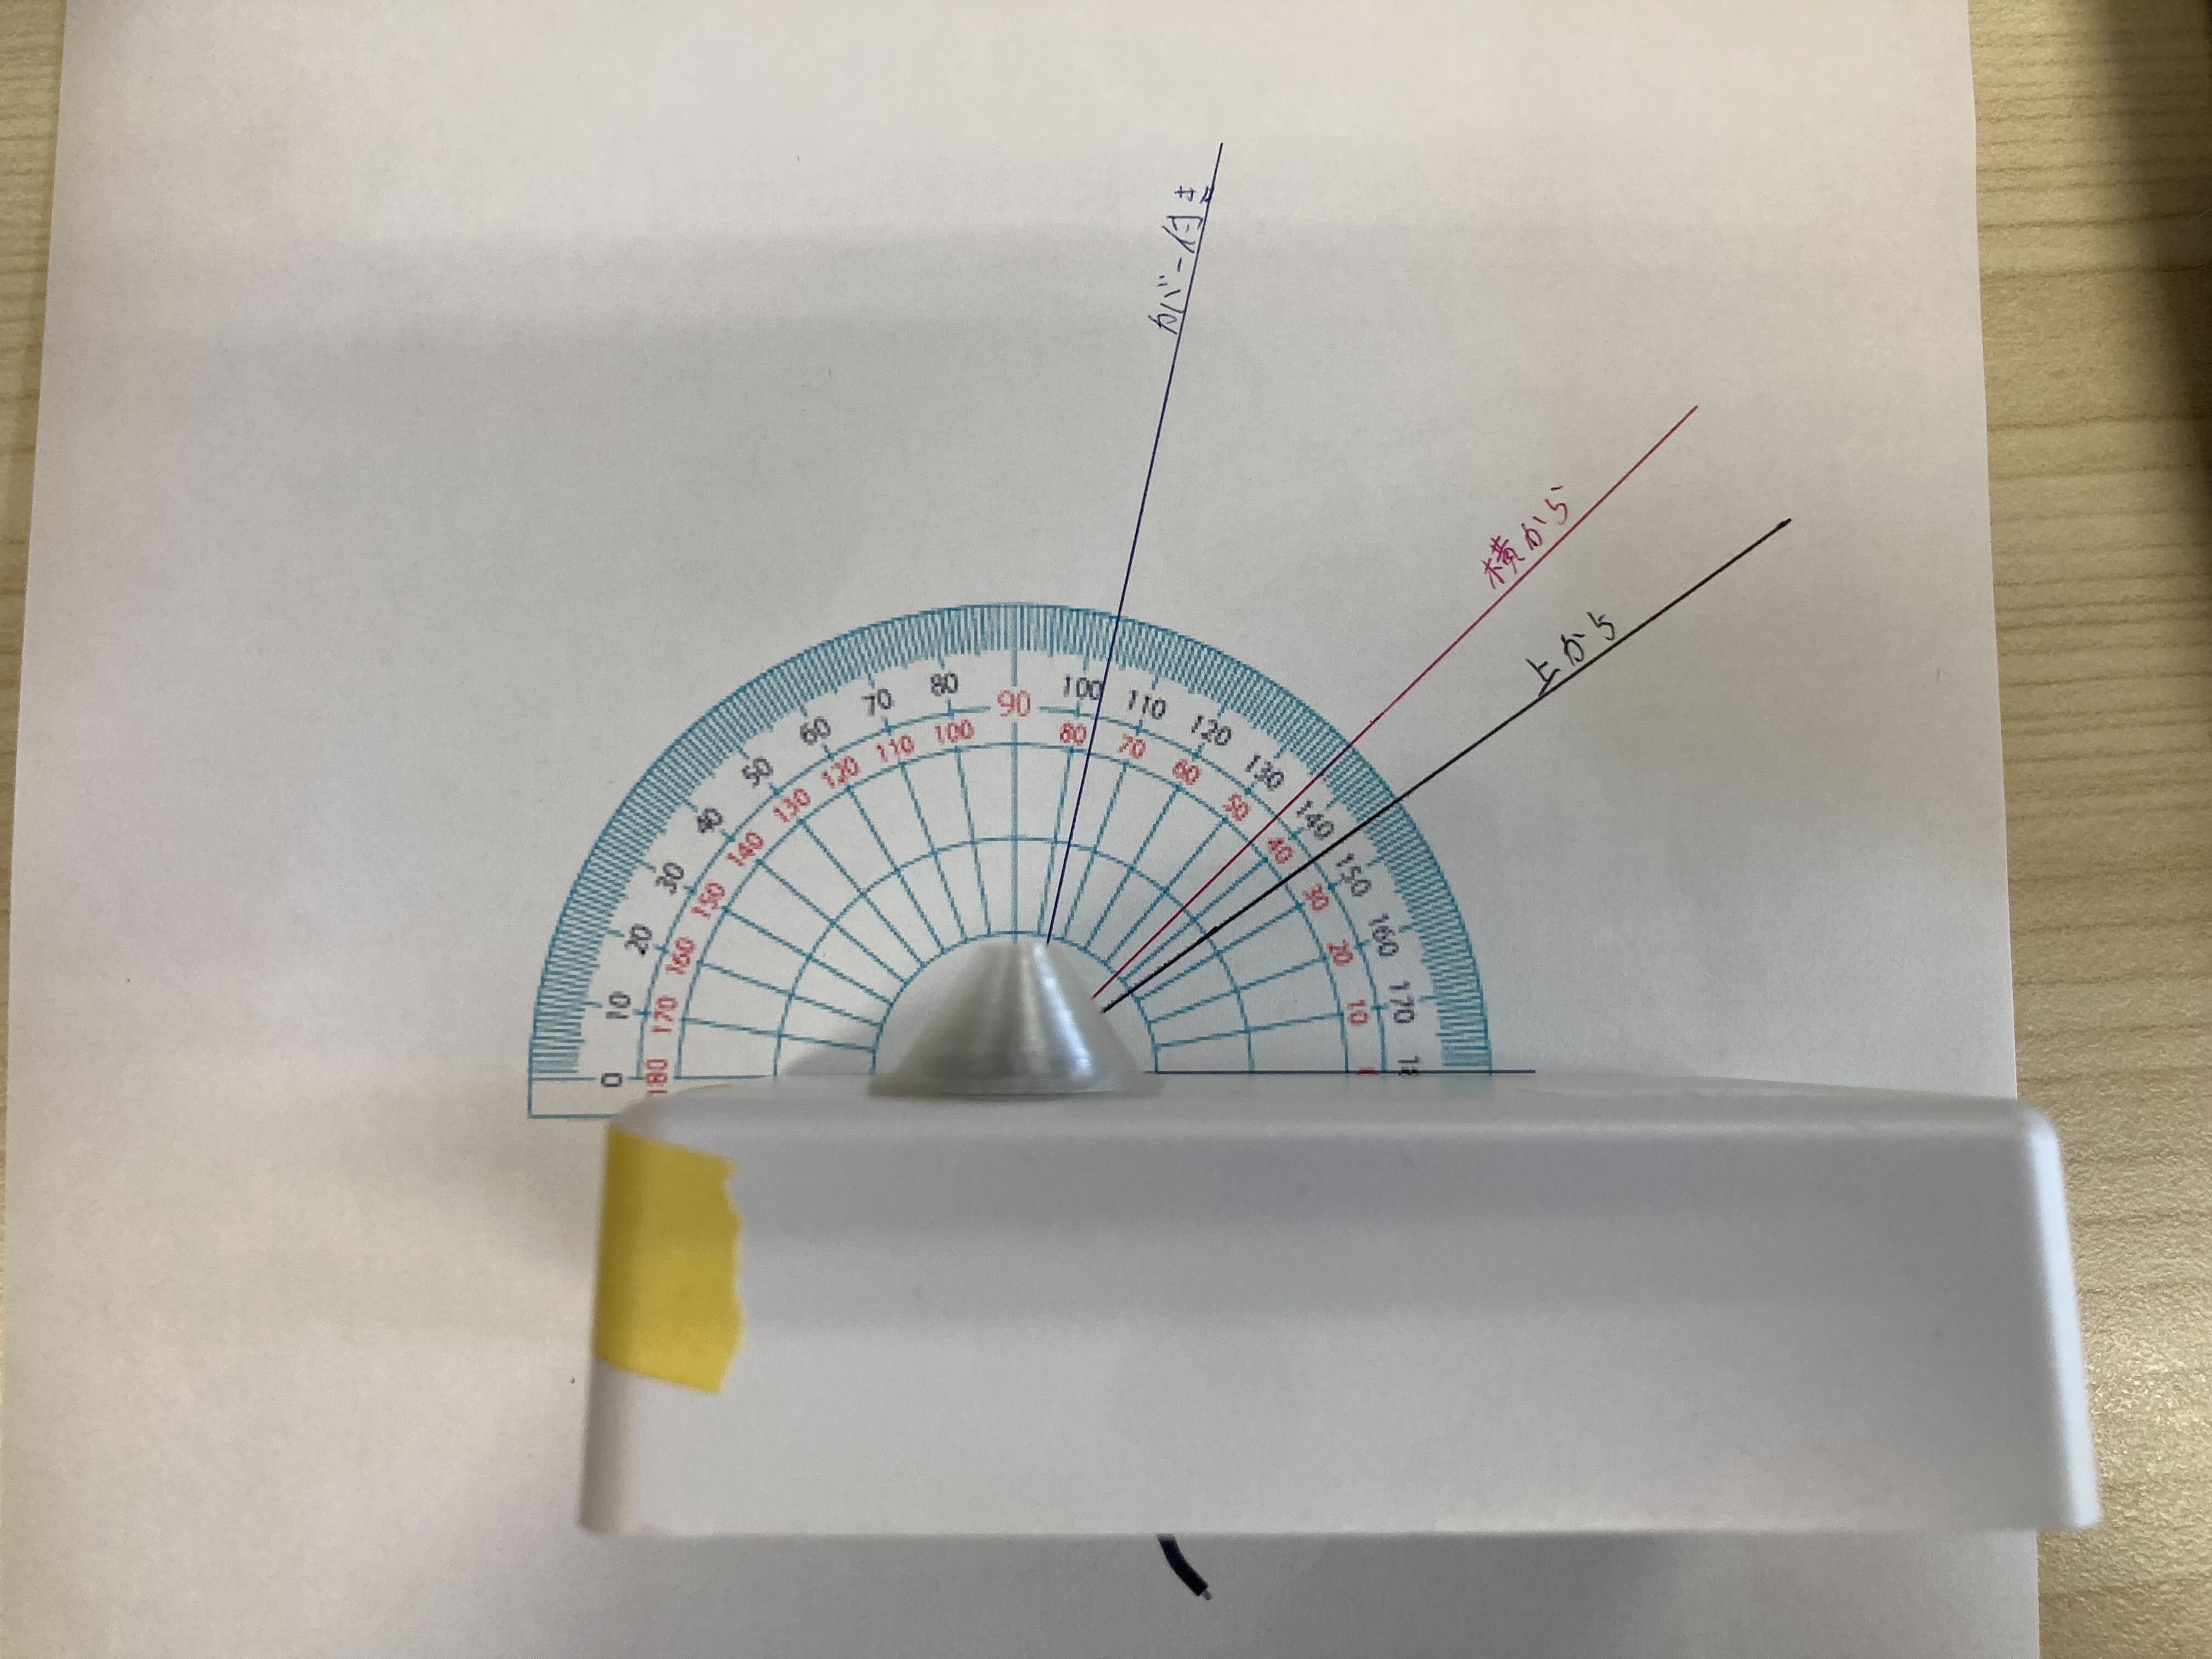
\includegraphics[width=.47\textwidth]{PIRsensor.jpg}
   \caption{センサのだいたいの検知範囲}
   \label{Fig:PIRsensor}
  \end{center}
\end{figure}

% -----------------------------------------------------------
% -----------------------------------------------------------

\begin{table}[h]
  \begin{center}
   \caption{センサの検知範囲}
   \label{Tab:range}
   \scalebox{1.1}[1.2]{
   \begin{tabular}{|c|c|c|c|}  \hline
    & \begin{tabular}{c}横から\end{tabular} & \begin{tabular}{c}上から\end{tabular} & \begin{tabular}{c}カバー有り\end{tabular}\\ \hline\hline
    角度 & 46度 & 56度 & 15\~{}20度\\ \hline
    \end{tabular}
   }
  \end{center}
\end{table}


\section{予定}
来週の予定
\begin{thebibliography}{9}
  \bibitem{1}
  パナソニック：焦電型赤外線センサ PaPIRs(パピルス)\par
  \url(https://industrial.panasonic.com/jp/products/pt/papirs/documents)
  \end{thebibliography}
\end{document}